\documentclass[12pt, oneside]{article}

\usepackage[letterpaper, scale=0.8, centering]{geometry}
\usepackage{fancyhdr}
\setlength{\parindent}{0em}
\setlength{\parskip}{1em}

\pagestyle{fancy}
\fancyhf{}
\renewcommand{\headrulewidth}{0pt}
\rfoot{{\footnotesize Copyright Mia Minnes, 2024, Version \today~(\thepage)}}

\usepackage{titlesec}

\author{CSE105W24}

\newcommand{\instructions}{{\bf For all HW assignments:} Weekly homework 
may be done individually or in groups of up to 3 students. 
You may switch HW partners for different HW assignments. 
Please ensure your name(s) and PID(s) are clearly visible on the first page of your homework submission 
and then upload the PDF to Gradescope. If working in a group, submit only one submission per group: 
one partner uploads the submission through their Gradescope account and then adds the other group member(s) 
to the Gradescope submission by selecting their name(s) in the ``Add Group Members" dialog box. 
You will need to re-add your group member(s) every time you resubmit a new version of your assignment.
 Each homework question will be graded either for correctness (including clear and precise explanations and 
 justifications of all answers) or fair effort completeness. 
 For ``graded for correctness''
 questions: collaboration is allowed only with CSE 105 students in your group; 
 if your group has questions about a problem, you may ask in drop-in 
 help hours or post a private post (visible only to the Instructors) on Piazza.
 For ``graded for completeness''
 questions: collaboration is allowed with any CSE 105 students this quarter; 
 if your group has questions about a problem, you may ask in drop-in 
 help hours or post a public post on Piazza.

All submitted homework for this class must be typed. 
You can use a word processing editor if you like (Microsoft Word, Open Office, Notepad, Vim, Google Docs, etc.) 
but you might find it useful to take this opportunity to learn LaTeX. 
LaTeX is a markup language used widely in computer science and mathematics. 
The homework assignments are typed using LaTeX and you can use the source files 
as templates for typesetting your solutions.
To generate state diagrams of machines, we recommend using Flap.js
or JFLAP. Photographs of clearly hand-drawn diagrams may also be used. We recommend that you
submit early drafts to Gradescope so that in case of any technical difficulties, at least some of your
work is present. You may update your submission as many times as you'd like up to the deadline.


{\bf Integrity reminders}
\begin{itemize}
\item Problems should be solved together, not divided up between the partners. The homework is
designed to give you practice with the main concepts and techniques of the course, 
while getting to know and learn from your classmates.
\item You may not collaborate on homework questions graded for correctness with anyone other than your group members.
You may ask questions about the homework in office hours (of the instructor, TAs, and/or tutors) and 
on Piazza (as private notes viewable only to the Instructors).  
You \emph{cannot} use any online resources about the course content other than the class material 
from this quarter -- this is primarily to ensure that we all use consistent notation and
definitions (aligned with the textbook) and also to protect the learning experience you will have when
the `aha' moments of solving the problem authentically happen.
\item Do not share written solutions or partial solutions for homework with 
other students in the class who are not in your group. Doing so would dilute their learning 
experience and detract from their success in the class.
\end{itemize}

}

\newcommand{\gradeCorrect}{({\it Graded for correctness}) }
\newcommand{\gradeCorrectFirst}{\gradeCorrect\footnote{This means your solution 
will be evaluated not only on the correctness of your answers, but on your ability
to present your ideas clearly and logically. You should explain how you 
arrived at your conclusions, using
mathematically sound reasoning. Whether you use formal proof techniques or 
write a more informal argument
for why something is true, your answers should always be well-supported. 
Your goal should be to convince the
reader that your results and methods are sound.} }
\newcommand{\gradeComplete}{({\it Graded for completeness}) }
\newcommand{\gradeCompleteFirst}{\gradeComplete\footnote{This means you will 
get full credit so long as your submission demonstrates honest effort to 
answer the question. You will not be penalized for incorrect answers. 
To demonstrate your honest effort in answering the question, we 
expect you to include your attempt to answer *each* part of the question. 
If you get stuck with your attempt, you can still demonstrate 
your effort by explaining where you got stuck and what 
you did to try to get unstuck.} }

\usepackage{tikz}
\usetikzlibrary{automata,positioning,arrows}

\usepackage{amssymb,amsmath,pifont,amsfonts,comment,enumerate,enumitem}
\usepackage{currfile,xstring,hyperref,tabularx,graphicx,wasysym}
\usepackage[labelformat=empty]{caption}
\usepackage{xcolor}
\usepackage{multicol,multirow,array,listings,tabularx,lastpage,textcomp,booktabs}

\lstnewenvironment{algorithm}[1][] {   
    \lstset{ mathescape=true,
        frame=tB,
        numbers=left, 
        numberstyle=\tiny,
        basicstyle=\rmfamily\scriptsize, 
        keywordstyle=\color{black}\bfseries,
        keywords={,procedure, div, for, to, input, output, return, datatype, function, in, if, else, foreach, while, begin, end, }
        numbers=left,
        xleftmargin=.04\textwidth,
        #1
    }
}
{}

\newcommand\abs[1]{\lvert~#1~\rvert}
\newcommand{\st}{\mid}

\newcommand{\cmark}{\ding{51}}
\newcommand{\xmark}{\ding{55}}
 
\newcommand{\SUBSTRING}{\textsc{Substring}}
\newcommand{\REP}{\textsc{Rep}}
\newcommand{\blank}{\scalebox{1.5}{\textvisiblespace}}
 
\title{HW3CSE105W24: Homework assignment 3}
\date{Due: February 15th at 5pm (no penalty late submission until 8am next morning), via Gradescope}


\begin{document}
\maketitle
\thispagestyle{fancy}

{\bf In this assignment,}

You will  practice with the definition of pushdown automata and context-free grammars and reason
about regular and context-free languages. You will also practice analyzing and designing Turing machines.

{\bf Resources}: To review the topics 
for this assignment, see the class material from Weeks 4-6.
We will post frequently asked questions and our answers to them in a 
pinned Piazza post.

{\bf Reading and extra practice problems}:  
Sipser Chapter 2, Section 3.1
Chapter 2 exercises 2.1, 2.2, 2.3, 2.4, 2.5, 2.6, 2.7, 2.9, 2.10, 2.11, 2.12, 2.13, 2.16, 2.17.
Chapter 3 exercises 3.1, 3.2. 

\instructions

You will submit this assignment via Gradescope
(\href{https://www.gradescope.com}{https://www.gradescope.com}) 
in the assignment called ``hw3CSE105W24''.

{\bf Assigned questions}
\begin{enumerate}[wide, labelwidth=!, labelindent=0pt]
\item \textbf{Constructions} (18 points):


Consider the push-down automata $M_1$ and $M_2$ over $\{a,b\}$ with stack alphabet $\{a, b\}$ whose state diagrams are

\begin{center}
\begin{multicols}{2}
    State diagram for $M_1$

    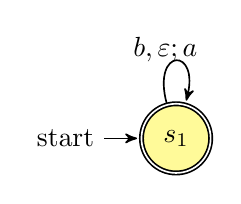
\begin{tikzpicture}[->,>=stealth',shorten >=1pt, auto, node distance=2cm, semithick]
    \tikzstyle{every state}=[text=black, fill=yellow!40]
    
    \node[initial,state, accepting] (s1)          {$s_1$};

    \path (s1) edge  [loop above, near start] node {$b,\varepsilon; a$} (s1)
    ;
    \end{tikzpicture}

    \columnbreak 

    State diagram for $M_2$

    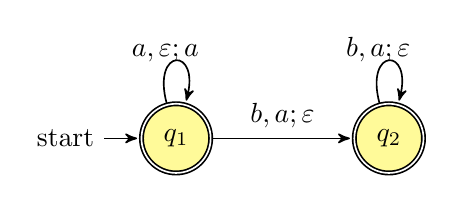
\begin{tikzpicture}[->,>=stealth',shorten >=1pt, auto, node distance=2cm, semithick]
    \tikzstyle{every state}=[text=black, fill=yellow!40]
    
    \node[initial,state, accepting] (q1)          {$q_1$};
    \node[state, accepting]         (q2) [right of=q1, xshift=20pt] {$q_2$};
    
    \path (q1) edge  [loop above, near start] node {$a,\varepsilon; a$} (q1)
        (q1) edge [bend left=0] node {$b,a;\varepsilon$} (q2)
        (q2) edge [loop above, near start] node {$b,a;\varepsilon$} (q2)
    ;
    \end{tikzpicture}
\end{multicols}
\end{center}
\begin{enumerate}
    \item \gradeCompleteFirst What is the language $A_1$ recognized by $M_1$ and what is the language $A_2$ recognized by $M_2$?
    Include a sample string that is accepted and one that is rejected for each of these PDA. Justify these examples
    with sample accepting computations or with an explanation why there is no accepting computation.
    \item \gradeCorrectFirst Design CFGs $G_1$ and $G_2$ over $\{a,b\}$ so that $L(G_1) = A_1$ and $L(G_2) = A_2$. A complete 
    solution will include precise definitions for each of the parameters required to specify a CFG, as well as a brief 
    explanation about why each string in $A_i$ can be derived in $G_i$ and each string not in $A_i$ cannot be derived in $G_i$ 
    (for $i=1,2$).
    \item \gradeComplete Remember that the definition of set-wise concatenation is:
    for languages $L_1, L_2$ over the alphabet $\Sigma$, we have the 
    associated set of strings
    \[
       L_1 \circ L_2 = \{ w \in \Sigma^* ~|~ w = uv \text{ for some strings } u \in L_1 \text{ and } v \in L_2 \}
    \]
    In class (and in the review quiz) we learned that the class of context-free languages is closed under set-wise concatenation.
    The proof of this closure claim using CFGs uses the construction: given $G_1 = ( V_1, \Sigma, R_1, S_1)$ and 
    $G_2 = (V_2, \Sigma, R_2, S_2)$ with $V_1 \cap V_2 = \emptyset$ and $S_{new} \notin V_1 \cup V_2$, define a new CFG
    $$G = (V_1 \cup V_2 \cup \{S_{new}\}, \Sigma, R_1 \cup R_2 \cup \{S_{new} \to S_1 S_2\}, S_{new})$$
    Apply this construction to your grammars from part (b) and give a sample derivation of a string in $A_1 \circ A_2$
    in this resulting grammar.
    \item \gradeCorrect If we try to extrapolate the construction that we used to prove that the class of regular languages
    is closed under set-wise concategation, we would get the following construction for PDAs: Given 
    $M_1 = (Q_1, \Sigma, \Gamma_1, \delta_1, q_1, F_1)$ and $M_2 = (Q_2, \Sigma, \Gamma_2, \delta_2, q_2, F_2)$
    with $Q_1 \cap Q_2 = \emptyset$, define $Q = Q_1 \cup Q_2$, $\Gamma = \Gamma_1 \cup \Gamma_2$, and
    $$M = (Q, \Sigma, \Gamma, \delta, q_1, F_2)$$ with 
    $\delta: Q \times \Sigma_\varepsilon \times \Gamma_\varepsilon \to \mathcal{P}(Q \times \Gamma_\varepsilon)$
    given by 
    $$\delta( q,a,b) = \begin{cases}
        \delta_1 (q,a,b) &\text{if $q \in Q_1 \setminus F_1$, $a \in \Sigma_\varepsilon$, $b \in {\Gamma_1}_\varepsilon$} \\
        \delta_2 (q,a,b) &\text{if $q \in Q_2$, $a \in \Sigma_\varepsilon$, $b \in {\Gamma_2}_\varepsilon$} \\
        \delta_1 (q,a,b) &\text{if $q \in F_1$, $a \in \Sigma$ or $b\in \Gamma_1$}\\
        \delta_1 (q,a,b) \cup \{ (q_2, \varepsilon)\} &\text{if $q \in F_1$, $a =\varepsilon$, $b=\varepsilon$}\\
        \emptyset &\text{otherwise}
    \end{cases}$$
    Apply this construction to the machines $M_1$ and $M_2$ from part (a), and then use the resulting PDA to prove that 
    {\it this} construction cannot be used to prove that the class of context-free languages is closed under set-wise
    concatenation. A complete solution will include (1) the state diagram of the machine $M$ that results from 
    applying this construction to $M_1$ and $M_2$, (2) an example of a string that is accepted by this PDA $M$ but that 
    is {\bf not} in the language $A_1 \circ A_2$ with a description of the computation that witnesses that this string 
    is accepted by $M$ and an explanation of why this string is not in $A_1 \circ A_2$ by referring back to the definitions
    of $A_1$, $A_2$, and set-wise concatenation.
\end{enumerate}

\item\textbf{Regular languages are context-free} (10 points):

Informally, we think of regular languages as potentially simpler than context-free languages. In this question, you'll make 
this precise by showing that every regular language is context-free, in two ways.
\begin{enumerate}
\item\gradeCorrect When we first introduced PDAs we saw that any NFA can be transformed to a PDA by not using the stack 
of the PDA at all. Make this precise by completing the following construction: Given a NFA $N = (Q, \Sigma, \delta_N, q_0, F)$
we define a PDA $M$ with $L(M) = L(N)$ by choosing \ldots
A complete solution will have precise, correct definitions for each of the defining parameters of $M$: the set of states,
the input alphabet, the stack alphabet, the transition function, the start state, and the set of accept states. Be careful
to use notation that matches the types of the objects involved.

\item\gradeCorrect In the book on page 107, the top paragraph describes a procedure for converting DFA to CFGs:
\begin{quote}
   You can convert any DFA into an equivalent CFG as follows. 
   Make a variable $R_i$ for each state $q_i$ of the DFA. Add the rule $R_i \to aR_j$ to the
   CFG if $\delta(q_i,a) =q_j$ is a transition in the DFA. Add the rule
   $R_i\to \varepsilon$ if $q_i$ is an accept state of the DFA. Make $R_0$ the start variable ofthe grammar, 
   where $q_0$ is the start state of the machine. Verify on your own that the resulting CFG 
   generates the same language that the DFA recognizes.
\end{quote}

Use this construction to get a context-free grammar generating the language 
\[
    \{ w \in \{0,1\}^* \mid w \text{ does not have $11$ as a substring}\}
\]
by (1) designing a DFA that recognizes this language and then (2) applying the construction from the book to convert the 
DFA to an equivalent CFG. A complete submission will include the state diagram of the DFA, a brief justification of why 
it recognizes the language, and then the complete and precise definition of the CFG that results from applying the construction 
from the book to this DFA. {\it Ungraded bonus: take a sample string in the language and see how the computation of 
the DFA on this string translates to a derivation in your grammar.}

\end{enumerate}


\begin{comment}
For any language $L \subseteq \Sigma^*$, recall that we define its \emph{complement} as 
$$\overline{L} := \Sigma^* - L = \{w \in \Sigma^* \mid w \notin L\}$$ That is, the complement of $L$ 
contains all and only those strings which are not in $L$. Our notation for regular expressions does not 
include the complement symbol. However, 
it turns out that the complement of a language described by a regular expression is guaranteed to also be describable by a 
(different) regular expression. For example, over the alphabet $\Sigma = \{0,1\}$, the complement of the language described 
by the regular expression $\Sigma^* 0$ is described by the regular expression $\varepsilon \cup \Sigma^*1$
because any string that does not end in $0$
must either be the empty string or end in $1$.

For each of the regular expressions $R$ over the alphabet $\Sigma = \{a,b\}$ below, write the regular 
expression for~$\overline{L(R)}$. Your regular expressions may use the symbols
$\varnothing$, $\varepsilon$, $a$, $b$, and the 
following operations to combine them: union, concatenation, 
and Kleene star.

Briefly justify why your solution for each part works by giving plain English descriptions of the language 
described by the regular expression and of its complement and connecting them to the regular 
expression via relevant definitions. An English description that is more 
detailed than simply negating the description in the original language will likely be helpful in the justification.

Alternatively, you can justify your solution by first designing a DFA that recognizes $L(R)$, 
using the construction from class and the book to modify this DFA to get a new DFA that recognizes~$\overline{L(R)}$, 
and then applying the constructions from class and the book to convert this new DFA to a regular expression.

For each part of the question, clearly state which approach you're taking and include enough intermediate
steps to illustrate your work.


\begin{enumerate}
    \item\gradeCorrect $a^*b^*$
    \item\gradeCorrect $(a \cup b) a b^*$
\end{enumerate}
\end{comment}

\item\textbf{Classifying languages} (12 points):
On page 4 of the week 4 notes, we have the following list of languages over the alphabet $\{a,b\}$

\begin{center}
\begin{tabular}{ccc}
    $\{a^nb^n \mid 0  \leq n  \leq 5 \}$
    &$\{b^n a^n \mid  n  \geq 2\}$
    &$\{a^m b^n \mid  0 \leq m\leq n\}$
\end{tabular}
\begin{tabular}{cc}
    $\{a^m b^n \mid  m \geq n+3,  n \geq 0\}$
    &$\{b^m a^n \mid  m \geq 1, n \geq  3\}$\\
    $\{ w  \in \{a,b\}^* \mid w = w^\mathcal{R} \}$
    &$\{ ww^\mathcal{R} \mid w\in \{a,b\}^* \}$ \\
\end{tabular}
\end{center}
\begin{enumerate}
    \item\gradeComplete Pick one of the regular languages and design a regular expression that describes it. 
    Briefly justify your regular expression by connecting
    the subexpressions of it to the intended language and referencing relevant definitions.
    \item\gradeComplete Pick another one of the regular languages and design a DFA that recognizes it. Draw the 
    state diagram of your DFA. Briefly justify your design by explaining the role each state plays in the machine, 
    as well as a brief 
    justification about how the strings accepted and rejected by the machine connect to the specified language.
    \item\gradeComplete Pick one of the nonregular languages and design a PDA that recognizes it. Draw the state diagram of 
    your PDA. Briefly justify your design by explaining the role each state plays in the machine, 
    as well as a brief 
    justification about how the strings accepted and rejected by the machine connect to the specified language.
    \item\gradeComplete Pick one of the nonregular languages and write a CFG that generates it. Briefly justify
    your design by by demonstrating how derivations in the grammar relate
    to the intended language.
\end{enumerate}

\item \textbf{Turing machines} (10 points):
Consider the Turing machine $T$ over the input alphabet $\Sigma = \{0,1\}$ with  the state
    diagram below (the tape alphabet is $\Gamma = \{ 0,1,X,\square\}$).  
    Convention: we do not include the node for the reject state $qrej$ and any missing transitions in the state diagram have value $(qrej,\square,R)$
    \begin{center}
    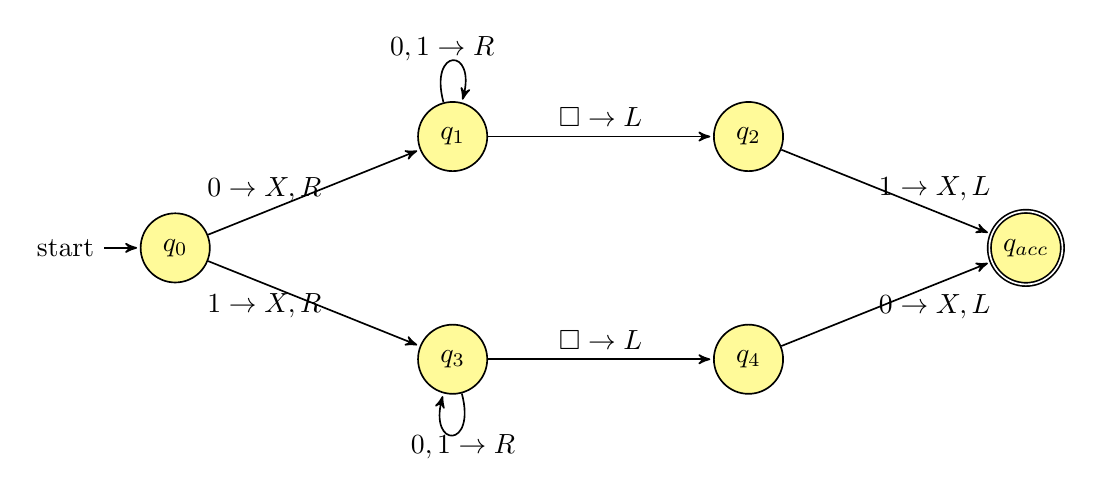
\begin{tikzpicture}[->,>=stealth',shorten >=1pt, auto, node distance=2cm, semithick]
        \tikzstyle{every state}=[text=black, fill=yellow!40]
        
        \node[initial,state] (q0)          {$q_0$};
        \node[state] (q1)  [above right of=q0, xshift=60pt] {$q_{1}$};
        \node[state] (q2)  [right of=q1, xshift=50pt] {$q_{2}$};
        \node[state] (q3)  [below right of=q0, xshift=60pt] {$q_{3}$};
        \node[state] (q4)  [right of=q3, xshift=50pt] {$q_{4}$};
        \node[state, accepting]         (qacc) [below right of=q2, xshift=60pt] {$q_{acc}$};
        
        \path (q1) edge  [loop above, near start] node {$0,1 \to R$} (q1)
            (q3) edge  [loop below, near start] node {$0,1 \to R$} (q3)
            (q0) edge [bend left=0, above, near start] node {$0\to X, R$} (q1)
            (q0) edge [bend left=0, below, near start] node {$1\to X, R$} (q3)
            (q1) edge [bend left=0] node {$\square \to L$} (q2)
            (q2) edge [bend left=0, above, near end] node {$1\to X, L$} (qacc)
            (q3) edge [bend left=0] node {$\square \to L$} (q4)
            (q4) edge [bend left=0, below, near end] node {$0\to X, L$} (qacc)
        ;
        \end{tikzpicture}
    \end{center}

    \begin{enumerate}

        \item\gradeCorrect Specify an example string $w_1$ of length $4$ over 
        $\Sigma$ that is {\bf accepted} by this Turing machine, or explain why there is no such 
        example. A complete solution will include either (1) a precise and clear 
        description of your example  string and a precise and clear description of the accepting computation
        of the Turing machine on this string or (2) a sufficiently
        general and correct argument why there is no such example, referring back to the relevant definitions.
        
        To describe a computation of a Turing machine, include the contents of the 
        tape, the state of the machine, and the location of the read/write head at each step in the computation.
        
        {\it Hint:} In class we've drawn pictures to represent the configuration of the machine at each step 
        in a computation.  You may do so or you may choose to describe these configurations in words.
        
        \item\gradeCorrect Specify an example string $w_2$ of length $3$ over $\Sigma$ 
        that is {\bf rejected} by this Turing machine
        or explain why there is no such 
        example. A complete solution will include either (1) a precise and clear 
        description of your example  string and a precise and clear description of the rejecting computation
        of the Turing machine on this string or (2) a sufficiently
        general and correct argument why there is no such example, referring back to the relevant definitions.

        \item\gradeCorrect Specify an example string $w_3$ of length $2$ over $\Sigma$ 
        on which  the computation of this Turing machine {\bf loops}
        or explain why there is no such 
        example. A complete solution will include either (1) a precise and clear 
        description of your example  string and a precise and clear description of the looping (non-halting) 
        computation
        of the Turing machine on this string or (2) a sufficiently
        general and correct argument why there is no such example, referring back to the relevant definitions.

        \item\gradeComplete Write an implementation level description of 
        the Turing machine $T$.
\end{enumerate}


\end{enumerate}
\end{document}